\begin{lemma}
    \label{lem:decomp_w_u}
    \ \newline
    \noindent
    \begin{minipage}{0.7\textwidth}
        Let $X$ be a graph. For a pushout square as shown on the right, we have 
        % $\card{\operatorname{Mono}(X, B)} \mathop{=} \card{\operatorname{Mono}(X, D, \beta')}$ and $\card{\operatorname{Mono}(X, C, \lnot \beta)} \mathop{=} \card{\operatorname{Mono}(X, D, \lnot \beta', \alpha')}$.
        \begin{flalign*}
            \card{\operatorname{Mono}(X, B)} &= \card{\operatorname{Mono}(X, D, \beta')}
            \\
            \card{\operatorname{Mono}(X, C, \lnot \beta)} &= \card{\operatorname{Mono}(X, D, \lnot \beta', \alpha')}
        \end{flalign*}
        
    \end{minipage}
    \hfill
    \begin{minipage}{0.3\textwidth}
        \hfill
        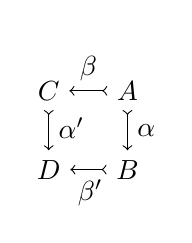
\begin{tikzpicture}
            \node (A) {$A$};
            \node [below of=A] (B) {$B$}; 
            \node [left of=A] (C) {$C$}; 
            \node [left of=B] (D) {$D$}; 
            \begin{scope}[nodes=rectangle]          
            \draw [>->] (A) to node [right,label,pos=0.5] {$\alpha$} (B);
            \draw [>->] (A) to node [above,label,pos=0.5] {$\beta$} (C);
            \draw [>->] (B) to node [below,label,pos=0.45] {$\beta'$} (D); 
            \draw [>->] (C) to node [right,label,pos=0.45] {$\alpha'$} (D);
            \end{scope}
        \end{tikzpicture}
    \end{minipage}
    \end{lemma}
    \begin{proof}
        \label{proof:dcomp_w_u}
    %    Since $\operatorname{Mono}(X, B) \mathop{=} \operatorname{Mono}(X, D, \beta')$ by definition of $\operatorname{Mono}(X, B)$ and $\operatorname{Mono}(X, D, \beta')$, the equality $\card{\operatorname{Mono}(X, B)} \mathop{=} \card{\operatorname{Mono}(X, D, \beta')}$ holds.
    \begin{claim}
        $\card{\operatorname{Mono}(X, B)} \mathop{=} \card{\operatorname{Mono}(X, D, \beta')}$
    \end{claim}
    \begin{itemize} 
        \item The inclusion \(\operatorname{Mono}(X, B) \mathop{\star} \beta' \mathop{\subseteq} \operatorname{Mono}(X, D, \beta')\) holds by definition of $\operatorname{Mono}(X, B)$ and $\operatorname{Mono}(X, D, \beta')$. 
        In fact, if \(\iota  \mathop{\in} \operatorname{Mono}(X, B) \mathop{\star} \beta' \), then there is a monomorphism \(\zeta : X \rightarrowtail B\) satisfying \(\iota \mathop{=} \zeta \mathop{\star} \beta'\). Since $\zeta \mathop{\star} \beta'$ is also a monomorphism\todo{monicity of $\beta'$}, \(\iota\) is also an element of \(\operatorname{Mono}(X, D, \beta')\).
        \item The inclusion \(\operatorname{Mono}(X, B) \mathop{\star} \beta' \supseteq \operatorname{Mono}(X, D, \beta')\) holds by definition of $\operatorname{Mono}(X, B)$ and $\operatorname{Mono}(X, D, \beta')$.
        Suppose \(\iota \mathop{\in} \operatorname{Mono}(X, D, \beta')\). There is a monomorphism \(\zeta : X \rightarrowtail B\) satisfying \(\iota \mathop{=} \zeta \mathop{\star} \beta'\). It follows that \(\iota \mathop{=} \zeta \mathop{\star} \beta' \mathop{\in} \operatorname{Mono}(X, B) \mathop{\star} \beta'\).
        \item Hence, we have \(\operatorname{Mono}(X, B) \mathop{\star} \beta' \mathop{=} \operatorname{Mono}(X, D, \beta')\).
        \item $\card{\operatorname{Mono}(X, B)} \mathop{=} \card{\operatorname{Mono}(X, D, \beta')}$ follows by the injectivity of $\beta'$\todo{monicity of $\beta'$}.
    \end{itemize}
    \begin{claim}
         $\card{\operatorname{Mono}(X, C, \lnot \beta)} \mathop{=} \card{\operatorname{Mono}(X, D, \lnot \beta', \alpha')}$
       \end{claim}
        \begin{itemize}
            % \item The inclusion \(\operatorname{Mono}(X, C, \lnot \beta) \mathop{\star} \alpha'  \mathop{\subseteq} \operatorname{Mono}(X, D, \lnot \beta', \alpha')\) can be justified as follows. Suppose that \(\iota : X \mathop{\to} D\) is an element of \(\operatorname{Mono}(X, C, \lnot \beta) \mathop{\star} \alpha'\). According to the definition of \(\operatorname{Mono}(X, C, \lnot \beta) \mathop{\star} \alpha'\), there exists \(\eta : X \mathop{\to} C\) in \(\operatorname{Mono}(X, C, \lnot \beta)\) such that \(\iota \mathop{=} \eta \mathop{\star} \alpha'\). We need to show that no \(\zeta : X \mathop{\to} B\) exists such that \(\iota \mathop{=} \zeta \mathop{\star} \beta'\). Assuming the contrary, that such a \(\zeta\) exists. Under this assumption, the following commutative diagram holds:
            \item The inclusion \(\operatorname{Mono}(X, C, \lnot \beta) \mathop{\star} \alpha'  \mathop{\subseteq} \operatorname{Mono}(X, D, \lnot \beta', \alpha')\) can be justified as follows: Suppose \(
                \eta \mathop{\star} \alpha' \mathop{\in} \operatorname{Mono}(X, C, \lnot \beta) \mathop{\star} \alpha'\).
            %  By the definition of \(\operatorname{Mono}(X, C, \lnot \beta) \mathop{\star} \alpha'\), there exists a morphism \(\eta : X \mathop{\to} C\) in \(\operatorname{Mono}(X, C, \lnot \beta)\) such that \(\iota \mathop{=} \). 
             Since $\eta \mathop{\star} \alpha'$ is a monomorphism\todo{monicity of $\alpha'$}, it suffices to show that there is no \(\zeta : X \rightarrowtail B\) such that \(\eta \mathop{\star} \alpha' \mathop{=} \zeta \mathop{\star} \beta'\). Suppose, by contradiction, that such a \(\zeta\) exists, then the following commutative diagram holds:
            \begin{center}
                \begin{tikzpicture}[node distance=10mm]
                    \node (A) {A}; 
                    \node (B) [above right=of A] {B};
                    \node (X) [left  = of A] {X};
                    \node (D) [below right=of B] {D};
                    \node (C) [below right=of A] {C};
                    \draw[>->] (A) to node[pos=.7, below] {$\alpha$} (B) ;
                    \draw[>->] (C) to  node[pos=0.7, below] {$\alpha'$} (D);
                    \draw[>->] (A) -- (C) node[pos=.4, right] {$\beta$};
                    \draw[>->] (B) -- (D) node[pos=.4, right] {$\beta'$};
                    \draw[>->] (X) -- node[above] {$\zeta$} (B);
                    \draw[>->] (X) -- node[below] {$\eta$} (C);
                \end{tikzpicture}
            \end{center} 
            The pushout square \(\square ABDC\) is also a pullback square, by Proposition~\ref{prop:pb_eq_po}. The universal property of the pullback provides a morphism \(\gamma : X \mathop{\rightarrow} A\) such that \(\eta \mathop{=} \gamma \mathop{\star} \beta\). \(\gamma\) is a monomorphism, because \(\eta \mathop{=} \gamma \mathop{\star} \beta\) and $\eta$ is a monomorphism. Therefore, the existence of $\gamma$ contradicts the assumption that \(\eta \mathop{\in} \operatorname{Mono}(X, C, \lnot \beta)\). Thus, \(\iota\) is also an element of \(\operatorname{Mono}(X, D, \lnot \beta', \alpha')\). 
            \item The inclusion \(\operatorname{Mono}(X, C, \lnot \beta) \mathop{\star} \alpha'  \supseteq \operatorname{Mono}(X, D, \lnot \beta', \alpha')\) can be justified as follows. Suppose that \(\iota : X \rightarrowtail D\) is an element of \(\operatorname{Mono}(X, D, \lnot \beta', \alpha')\). According to the definition of \(\operatorname{Mono}(X, D, \lnot \beta', \alpha')\), there exists \(\eta : X \rightarrowtail C\) making 
                \begin{flalign}
                    \iota \mathop{=} \eta \mathop{\star} \alpha' \label{eq:etastaralphap}
                \end{flalign}
            We show that \(\eta\) is an element of 
            \(\operatorname{Mono}(X, C, \lnot \beta)\) by contradiction.
            
            Suppose that there is a monomorphism \(\zeta : X \rightarrowtail A\) such that 
            \begin{flalign}
                \eta \mathop{=} \zeta \mathop{\star} \beta \label{eq:zetastarbeta}
            \end{flalign}
            and observe:
            \begin{flalign*}
               \hspace{2cm} \iota &\overset{\operatorname{def}}{=} \eta \mathop{\star} \alpha' &\text{by Equation~\eqref{eq:etastaralphap}} 
               \\
                      &\overset{\operatorname{def}}{=} (\zeta \mathop{\star} \beta) \mathop{\star} \alpha' & \text{by Equation~\eqref{eq:zetastarbeta}}
                      \\
                      &= \zeta \mathop{\star} (\beta \mathop{\star} \alpha') & \text{by associativity} 
                      \\
                      &= \zeta \mathop{\star} (\alpha \mathop{\star} \beta') &\text{by commutativity of $ABDC$}\\
                      &= (\zeta \mathop{\star} \alpha) \mathop{\star} \beta'
            \end{flalign*}
              There is a contradiction because no such factorization of \(\iota\) should exist as \(\iota \mathop{\in} \operatorname{Mono}(X, D, \lnot \beta', \alpha')\).
            %    Therefore, there is no \(\zeta : X \mathop{\rightarrow} A\) such that \(\eta \mathop{=} \zeta \mathop{\star} \beta\), confirming \(\eta\) as an element of \(\operatorname{Mono}(X, C, \lnot \beta)\). Consequently, \(\iota \mathop{=} \eta \mathop{\star} \alpha'\) is an element of \(\operatorname{Mono}(X, C, \lnot \beta) \mathop{\star} \alpha'\).
            \item We conclude by the monicity of \(\alpha'\). \todo{monicity of $\alpha'$}
            % From \(\operatorname{Mono}(X, C, \lnot \beta) \mathop{\star} \alpha'  \mathop{\subseteq} \operatorname{Mono}(X, D, \lnot \beta', \alpha')\) and \(\operatorname{Mono}(X, C, \lnot \beta) \mathop{\star} \alpha'  \supseteq \operatorname{Mono}(X, D, \lnot \beta', \alpha')\), we conclude \(\operatorname{Mono}(X, C, \lnot \beta) \mathop{\star} \alpha' \mathop{=} \operatorname{Mono}(X, D, \lnot \beta', \alpha')\) and \(\card{\operatorname{Mono}(X, C, \lnot \beta) \mathop{\star} \alpha'} \mathop{=} \card{\operatorname{Mono}(X, D, \lnot \beta', \alpha')}\).
            % Since \(\alpha'\) is monic, \(\card{\operatorname{Mono}(X, C, \lnot \beta)} \mathop{=} \card{\operatorname{Mono}(X, C, \lnot \beta) \mathop{\star} \alpha'}\). Therefore, \(\card{\operatorname{Mono}(X, C, \lnot \beta)} \mathop{=} \card{\operatorname{Mono}(X, D, \lnot \beta', \alpha')}\).
        \end{itemize}
    \end{proof} 
    
    \begin{lemma}
        \label{lem:xlnlmxrnr}
        Let $X$ be a graph. Let $L \overset{l}{\leftarrow} K \overset{r}{\rightarrow} R$ be an injective DPO graph rewriting rule. We have 
        \[
            \card{\operatorname{Mono}(X, L, \lnot l)}  - \card{\operatorname{Mono}(X, R, \lnot r)} 
            \mathop{=} 
            \card{\operatorname{Mono}(X, L)}  - \card{\operatorname{Mono}(X, R)} 
        \]
    \end{lemma}
    \begin{proof}
        \label{proof:lem:xlnlmxrnr}
        
        \begin{claim}
           $\card{\operatorname{Mono}(X, L, l)} \mathop{=} \card{\operatorname{Mono}(X, R, r)}$
        \end{claim}
        \begin{itemize}
            \item We prove $\card{\operatorname{Mono}(X, L, l)} \leq \card{\operatorname{Mono}(X, R, r)}$ by constructing an injection from $\operatorname{Mono}(X, L, l)$ to $\operatorname{Mono}(X, R, r)$. Let $h \mathop{\in} \operatorname{Mono}(X, L, l)$. By definition, we have $h \mathop{=} g \mathop{\star} l$ for some $g: X \rightarrowtail K$. Thus, $g \mathop{\star} r \mathop{\in} \operatorname{Mono}(X, L, r)$. Let $h' \mathop{\in} \operatorname{Mono}(X, L, l)$ such that $h \mathop{\neq} h'$. We have $h' \mathop{=} g' \mathop{\star} l$ for some $g':X \rightarrowtail K$. We have $g \mathop{\neq} g'$ because otherwise we would have $h \mathop{=} g \mathop{\star} l \mathop{=} g' \mathop{\star} l \mathop{=} h'$. From the monicity of $r$, we conclude $g \mathop{\star} r \mathop{\neq} g' \mathop{\star} r$.
            \item Analoguously, we can prove $\card{\operatorname{Mono}(X, L, l)} \mathop{\geq} \card{\operatorname{Mono}(X, R, r)}$ by constructing an injection from $\operatorname{Mono}(X, R, r)$ to $\operatorname{Mono}(X, L, l)$.
            %  Let $h \mathop{\in} \operatorname{Mono}(X, R, r)$. By definition, we have $h \mathop{=} g \mathop{\star} r$ for some $g: X \rightarrowtail K$. Thus, $g \mathop{\star} l \mathop{\in} \operatorname{Mono}(X, L, l)$.
            % Let $h' \mathop{\in} \operatorname{Mono}(X, R, r)$ such that $h \mathop{\neq} h'$. We have $h' \mathop{=} g' \mathop{\star} l$ for some $g':X \rightarrowtail K$. Since $r$ is monic, we deduce $g \mathop{\neq} g'$. From the monicity of $l$, we conclude $g \mathop{\star} r \mathop{\neq} g' \mathop{\star} r$.
        \end{itemize}
        Hence, the following equality holds
        \begin{flalign*}
             &\card{\operatorname{Mono}(X, L, \lnot l)}  - \card{\operatorname{Mono}(X, R, \lnot r)}\\
            =&\card{\operatorname{Mono}(X, L) \mathop{\setminus} \operatorname{Mono}(X, L, l)}  - 
                \card{\operatorname{Mono}(X, R) \mathop{\setminus} \operatorname{Mono}(X, R, r)}\\
            =&(\card{\operatorname{Mono}(X, L)} - \card{\operatorname{Mono}(X, L, l)}) - (\card{\operatorname{Mono}(X, R)} - \card{\operatorname{Mono}(X, R, r)}) \\
            =&(\card{\operatorname{Mono}(X, L)} - \card{\operatorname{Mono}(X, R)})
             - (\card{\operatorname{Mono}(X, L, l)} - \card{\operatorname{Mono}(X, R, r)})\\
            \mathop{=} &\card{\operatorname{Mono}(X, L)} - \card{\operatorname{Mono}(X, R)}
        \end{flalign*}
    \end{proof}

